As a starting point in our quest for a fast kNN search, we investigated relevant literature. Consulting our advisors lead us to two papers by Garcia et.al. \citep{Garcia2008, Garcia2010}. In these papers, a parallel brute-force algorithm is developed, capable of solving the kNN problem orders of magnitude faster than comparable fast serial algorithms. Unfortunately, the algorithm developed by Garcia et.al. has some limitations, especially regarding the number of points that the kNN problem can be solved for. This could be due to the general nature of the algorithm developed by Garcia et.al. as it is optimized for solving problems in a large number of dimensions. By optimizing the algorithm for point cloud data, we could be able to get around this limitation.

\begin{myrq}
    Can high performance be achieved by a parallel brute-force kNN algorithm on large point clouds.
    \label{rq:brute_force_performance}
\end{myrq}

Given a fast kNN algorithm for point cloud data, the All-kNN problem can be solved easily, by applying the algorithm sequentially for all points in the cloud. This, however, is a strategy sensitive to minor inefficiencies in the kNN algorithm. The algorithm will have to be very fast for a single problem, in order to solve the All-kNN problem within reasonable time. Whether this is achievable with a fast brute-force based algorithm will have to be investigated.

\begin{myrq}
    Can a parallel brute-force kNN algorithm be fast enough to solve the All-kNN problem within reasonable time?
    \label{rq:brute_force_Q-kNN}
\end{myrq}

\subsection{Progress made by Garcia et.al.} % (fold)
\label{sub:garcia_s_effort}

The algorithm developed by Garcia et.al. is general in nature, and solves the kNN problem for any given dimension. It does this by performing the following three steps:

\begin{enumerate}
       \item Compute all distances between the query point $q$, and all reference points in $S$.
       \item Sort the distances.
       \item Pick the $k$ shortest distances.
\end{enumerate}

If this general brute-force algorithm is to be used on $n$ query points the time complexity will be \BigO{n\ m\ d}. To an experienced programmer, this might seem like a inefficient choice for a kNN algorithm. Usually, brute-fore based algorithm is  frowned upon, but when taking into account parallelization, it can be a valid choice. Brute-force algorithms tend to perform a lot of isolated computations, which can be easily parallelized. Combined with potential poor performance of the serial brute-force algorithm, this gives great speedup, and in some cases actual good performance. In addition brute-force algorithms tend to be very robust on different data, and behave in a predictable manner.
% subsection garcia_s_effort (end)

\subsection{Optimizing the brute-force algorithm for point cloud data} % (fold)
\label{sub:continuing_on_garcia_s_path} 

In order to improve performance of the general brute-force algorithm, we want restrict it to 3D space, and optimize it for low values of $k$. We also want to iron out any implementation choices made, that limit the number of points, $m$, the algorithm can operate on. Let us start by addressing the limit on number of points.

The implementation made by Garcia et.al. only supports problem sizes up to $65535$. The limitation of $65535$ corresponds to the number of theoretical blocks a CUDA kernel is allowed to spawn. This limitation is therefore only an implementation issue, not an issue with the underlying algorithm, and can be solved by applying a general partitioning algorithm. This algorithm splits the work amongst different CUDA blocks, and is shown in Algorithm~\ref{alg:general_aspects_dividing}.

\begin{algorithm}[ht]
\caption{General work distribution in CUDA}
\label{alg:general_aspects_dividing}
\begin{algorithmic}
\State Let $L$ be any dividable work quantity of size $l$.
    \Function{CUDA-Kernel}{$L$}
    \State $b \gets blockIdx.x$ \Comment{Current block id.}
    \State $d \gets gridDim.x$ \Comment{Numbers of theoretical blocks in current grid.}
    \While{$b<l$}
    \State \Call{do-work}{$L(b)$}
    \State $b \gets b + d$
    \EndWhile
    \EndFunction
\end{algorithmic}
\end{algorithm}

Additional improvements can be made to the general base algorithm, if we take advantage of our restrictions to the kNN problem. With the dimension fixed to three, the Euclidean distance can be calculated in a more optimized fashion. CUDA consists of lightweight threads, which makes reducing the amount of arithmetic calculations important for achieving good performance. The general base algorithm, who has to take any number of dimensions into account, uses two vectors and cuBlas to calculate the distance. This increases the complexity and data bandwidth required, and can be removed in our case.

The final, and maybe the most important, optimization we want to make, is changing the sorting operation, used to sort the computed distances. For problem instances in a low number of dimensions, the most time consuming operation is the sorting operation. For instance, given a search with $8$ dimensions, the sort consumes $62\%$ of the runtime \cite{Garcia2008}.

\subsubsection{Bitonic sort} % (fold)
\label{ssub:bitonic_sort}

It is proven that general sorting can be performed with a time complexity of \BigO{m\ log(m)} \cite{Cormen:2001}. This is a costly operation, if one only need the smallest $k$ values in a list, as is the case with the brute-force algorithm. To improve this, a sorting algorithm that sorts the list in a linear fashion, where the smallest elements are sorted first, could be used. This strategy is applied to the general brute-force algorithm.

However, using this strategy often forces us to select a sorting algorithm with bad time complexity. For instance, the insertion sort algorithm, used in the general brute-force algorithm \cite{Cormen:2001}, has a time complexity of \BigO{m^2}, the time complexity of finding the $k$ smallest points will therefore be \BigO{m\ k}. Asymptotically, this would give better timing results in cases where $k$ is smaller then $log(m)$. Let us analyze a case with $k=100$. For the insertion sort to get any asymptoticly advantage over the best sorting algorithms, the problem size has to be larger than $2^{100}$, which requires a point cloud of $1.3e30$. This is unrealistic for our problem. Choosing another sorting algorithm could therefore be a better strategy.

Graham Nolan discusses the possibility of improving Garcia's algorithm by using bitonic sort, and he states that it gives a significant improvement \citep{Nolan}. Bitonic sort is a known \BigO{m\ log(m)} algorithm, and is based around a soring network. The network is a series of interleaving bitonic sequences. A sequence is bitonic if it monotonically increases and then monotonically decreases \cite{Cormen:2001}. An iterative version of the bitonic sort is described in Algorithm~\ref{alg:bitonic_sort}.

\begin{algorithm}[ht]
\caption{Iterative Bitonic sort}
\label{alg:bitonic_sort}
\begin{algorithmic}
    \Require{A list $L$ with length $m$.}
    \Ensure{A sorted list, $L$}
    \State $P \gets \{2^i|i \in \mathcal{N} \}$
    \Function{Bitonic-Sort}{$L$}
        \ForAll{$\{p \in P\ |\ p \le m \}$}
            \ForAll{ $\{k \in P\ |\ p \ge k > 0\}$}
                \ForAll{$0 \le i < m)$}
                \State $pos \gets k \veebar p$ \Comment{$\veebar$ is the bitwise $xor$ operator}
                \If{$pos < i$}
                    \If{$\lnot(i \& p)$} \Comment{$\&$ is the bitwise $and$ operator}
                        \State \Call{compare}{$L(i),L(pos)$}
                    \EndIf
                    \If{$(i \& p)$}
                        \State \Call{compare}{$L(pos),L(i)$}
                    \EndIf
                \EndIf
                \EndFor
            \EndFor
        \EndFor
    \EndFunction
    \Statex
    \Function{Compare}{$a,b$}
    \If{$a>b$}
    \State \Call{swap}{$a,b$}
    \EndIf
    \EndFunction
\end{algorithmic}
\end{algorithm}
% subsubsection bitonic_sort (end)

\subsubsection{Min-reduce} % (fold)
\label{ssub:min_reduce}

Sorting the distances, with a \BigO{m\ log(m)} time complexity, still looks like a high price to pay to get the smallest values. Especially if $k$ is reasonably small. Do we need to sort the list in the first place? An algorithm that is more suitable, and also highly parallelizable, is the reduce operation. Cormen \cite{Cormen:2001} defines $\otimes$-reduction of an array $d$ of size $m$, where $\otimes$ is any associative operator, to be the value $y$, given by the following formula:

     $$ y = d[1] \otimes d[2] \dots \otimes d[m].$$

In the serial case, this is a typical linear algorithm with time complexity \BigO{m}, as shown in Algorithm~\ref{alg:serial_reduce}. 

\begin{algorithm}[ht]
\caption{Serial $\otimes$-reduction}
\label{alg:serial_reduce}
\begin{algorithmic}
    \State Let $\otimes$ be any associative operator.
    \Function{Reduce}{$d, \otimes$}
        \State $y \gets d[0]$
        \For{$i \gets 1,\, m$}
            \State $y \gets y \otimes d[i]$
        \EndFor
    \EndFunction
\end{algorithmic}
\end{algorithm}

Since the operator $\otimes$ is associative, there is no difference in which way the values are calculated or if it's done on parallel. A tree based approach, like Figure~\ref{fig:paralell_reduce_operation}, could be used. It is a good parallelization strategy, where every possible independent subtask is parallelized. Here each tree level do the associative operations in parallel, the results are combined as the tree level progresses downwards, until only one element remains. The parallel equivalent to Algorithm~\ref{alg:serial_reduce} is therefore done in \BigO{log(n)} time. 

\begin{figure}[ht!]
\centering
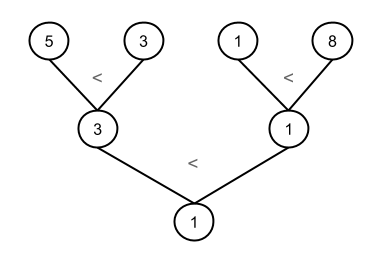
\includegraphics[width=50mm]{../gfx/min_reduce.png}
\caption{A visualization of the parallel min-reduce operation.}
\label{fig:paralell_reduce_operation}
\end{figure}

To solve our problem the associative operation has to be the minimum operator. Implementing the min-reduce algorithm can easily be done in CUDA, but in order to get the best performance some optimization techniques, like loop unrolling, sequential addressing and warp unrolling, described in Section~\ref{sec:cuda_optimizations} should be applied.   
% subsubsection min_reduce (end)

\subsubsection{Results} % (fold)
\label{ssub:comparison}

Two variations of our restricted brute-force algorithm where implemented, one using the bitonic-sort strategy, and one using the min-reduce operator. Both where compared to the algorithm developed by Garcia et.al\@. The complete implementations can be found in Appendix~\ref{sec:brute_force_garcia}

Figure~\ref{fig:brute_force} shows the timing results with $k$ equals $10$, for the three different brute-force implementations.

We see that the general brute-force algorithm has the worst performance. This is as expected, since it is developed for solving a more general problem, and does not use the optimizations described in our previous sections. The results for the brute-force implementation using bitonic sort, shows that Graham Nolan's idea of improving the sorting algorithm give a huge impact. It is almost five times faster then Garcia's implementation, shown in Table~\ref{tab:tabulated_results_from_brute_force}. As a note, bitonic sort has a soring network that is most suited for lengths that is a power of two. This explains the two drops observed in the graph.

\begin{figure}[ht!]
\centering
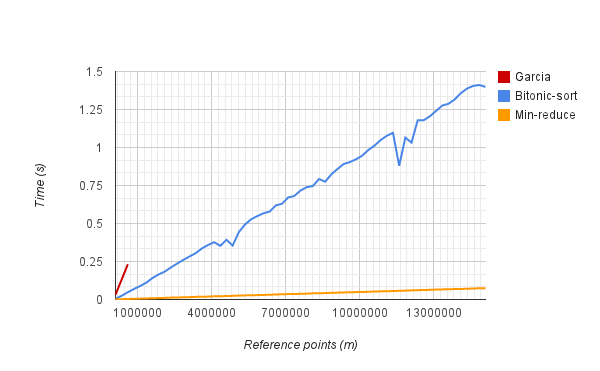
\includegraphics[width=100mm]{../gfx/brute_force.png}

\caption{Three different kNN brute-force implementations. The timing results is based on a $k$ equal to $10$.}
\label{fig:brute_force}
\end{figure}

\begin{table}[ht]
\centering
    \begin{tabular}{ | l | l |l |l|}
    \hline
    \textbf{Reference points (m)} &\textbf{Garcia} & \textbf{Bitonic sort} & \textbf{Min-reduce}\\ \hline
    \textbf{\numprint{6.0e5}} & $231.8ms$ & $48.1ms$& $3.3ms$\\ \hline
    \textbf{\numprint{1.1e7}} & -& $1077.2ms$ & $54.2 ms$ \\ \hline
    \end{tabular}
    \caption{Selected results from Figure~\ref{fig:brute_force}.}
    \label{tab:tabulated_results_from_brute_force}
\end{table}

The big winner in this comparison is the min-reduce version. It is $70$ times faster than the general brute-force algorithm, and almost $15$ times faster then the bitonic version.

Although the min-reduce brute-force algorithm is the best choice in this test for low values of $k$, this is not always the case. Performing $k$ min-reduce operations takes \BigO{k\ log(m)} time, because one min-reduce has a time complexity of \BigO{log(m)}. If we increase $k$ towards $m$, the result would be a sorted list, and the time complexity will go towards \BigO{m\ log(m)}. This is the same time complexity as our bitonic sort, but a sorting operation with min-reduce have a bigger constant time penalty than the bitonic version. However, for our use case, where $k$ is kept reasonably small, the min-reduce method is far superior.
% subsubsection comparison (end)
 % subsection garcia_s_effort (end) 
